\documentclass[12pt]{article}
\usepackage[utf8]{inputenc}
\usepackage{amsmath}
\usepackage{amsfonts}
\usepackage{amssymb}
\usepackage{graphicx}
\usepackage{subcaption}
\usepackage{cite}
\usepackage{url}

\usepackage{setspace}
\onehalfspacing

\title{Venture Capital Network Structure and Nestedness Analysis}
\author{}
\date{}

\begin{document}

\maketitle

\section{Methodology}

\subsection{Data Source and Preprocessing}

This study uses data from Crunchbase, a broad database containing information about startups, venture capital firms, and investment rounds. The dataset includes information about companies, investors, investments, and funding rounds in the United States market. International venture capital firms from other countries also appear in the dataset when they participate in US startup investments.

The data preprocessing follows established methodologies from entrepreneurship literature \cite{Dalle2025}. The cleaning process implemented includes several steps: (1) removal of companies with incomplete information, (2) exclusion of companies founded after 2017 to allow sufficient time for investment patterns to emerge, (3) removal of companies with exit status (bankruptcy, acquisition, or IPO), and (4) application of a minimum funding threshold of \$150,000 to focus on substantive investment relationships.

@todo: maybe remove following paragraph

To avoid endogeneity bias, companies that received funding only from accelerators were excluded from the analysis, following the approach described by Dalle et al. \cite{Dalle2025}. This ensures that observed network patterns reflect genuine investor relationships rather than program-specific effects.

\subsection{Investment Network Construction}

The analysis focuses on venture capital co-investment patterns across different funding stages. Investment stages are categorized into two main groups:
\begin{itemize}
    \item Early stages: angel, pre-seed, seed, and Series A
    \item Late stages: Series B through Series I
\end{itemize}

A bipartite network is constructed where nodes represent venture capital firms and edges represent co-investment relationships in the same company. The network is bipartite because it connects two distinct sets of investors: those participating in early-stage rounds (right nodes) and those participating in late-stage rounds (left nodes).

This approach allows us to study how early-stage and late-stage investors interact in the investment ecosystem.

The bipartite graph $G = (U \cup V, E)$ consists of:
\begin{align}
U &= \{u_1, u_2, \ldots, u_m\} \text{ (late-stage VCs)} \\
V &= \{v_1, v_2, \ldots, v_n\} \text{ (early-stage VCs)} \\
E &\subseteq U \times V \text{ (co-investment relationships)}
\end{align}

To prevent spurious connections from related entities, investor pairs where the first five characters of their names match are filtered out, reducing the likelihood of including different funds from the same parent organization. Further more,  Investors that participated in both early and late stages receive a suffix so they can be threated as distinct agents for each phase.

\subsection{Community Detection}

Community structure in the bipartite network is identified using the greedy modularity optimization algorithm \cite{Borgatti2011}. This method iteratively merges communities to maximize the modularity score, which measures the density of connections within communities compared to connections between communities.

For a bipartite network, modularity $Q$ is defined as:
\begin{equation}
Q = \frac{1}{2m} \sum_{i,j} \left[ A_{ij} - \frac{k_i k_j}{2m} \right] \delta(c_i, c_j)
\end{equation}

where $A_{ij}$ is the adjacency matrix, $k_i$ is the degree of node $i$, $m$ is the total number of edges, $c_i$ is the community of node $i$, and $\delta(c_i, c_j)$ is 1 if nodes $i$ and $j$ are in the same community, 0 otherwise.

The algorithm identifies communities of venture capital firms that frequently co-invest together, revealing structural patterns in the investment ecosystem that may not be apparent from individual investment decisions.

\subsection{Nestedness Analysis}

Nestedness is a structural property commonly observed in ecological networks \cite{AlmeidaNeto2008} that describes the tendency for specialists to interact with a subset of the partners of generalists. In the context of venture capital networks, nestedness would indicate that investors with fewer connections tend to co-invest with a subset of the partners of more connected investors.

We measure nestedness using the NODF (Nestedness based on Overlap and Decreasing Fill) metric \cite{AlmeidaNeto2008}. For a bipartite adjacency matrix $M$ with rows and columns sorted by decreasing degree, NODF is calculated as:

\begin{equation}
NODF = \frac{NODF_{rows} + NODF_{columns}}{2}
\end{equation}

where:
\begin{align}
NODF_{rows} &= \frac{100}{R(R-1)/2} \sum_{i=1}^{R-1} \sum_{j=i+1}^{R} \frac{|N_i \cap N_j|}{k_j} \text{ if } k_i > k_j \\
NODF_{columns} &= \frac{100}{C(C-1)/2} \sum_{i=1}^{C-1} \sum_{j=i+1}^{C} \frac{|N_i \cap N_j|}{k_j} \text{ if } k_i > k_j
\end{align}

Here, $R$ and $C$ are the number of rows and columns, $N_i$ represents the set of connections for node $i$, and $k_i$ is the degree of node $i$.

With this method, NODF vary between 0 and 1 (perfect nestedness).

\subsection{Statistical Significance Testing}

To determine whether observed nestedness values are significantly higher than expected by chance, we employ a null model approach using the Curveball algorithm \cite{Strona2014}. This algorithm generates randomized matrices that preserve the degree sequence of both node sets while randomizing the connection patterns.

For each community, we generate 100 null matrices (@todo: generate 1000 instead) using 10,000 Curveball iterations. The statistical significance is assessed by comparing the observed NODF score against the distribution of null model scores:

\begin{equation}
Z = \frac{NODF_{observed} - \mu_{null}}{\sigma_{null}}
\end{equation}

where $\mu_{null}$ and $\sigma_{null}$ are the mean and standard deviation of the null distribution. Communities with $p < 0.05$ (where $p$ is the proportion of null models with NODF $\geq$ observed NODF) are considered to have significantly high nestedness.

\section{Results}

\subsection{Network Characteristics}

\newcommand{\numCompanies}{22,527}
\newcommand{\numInvestors}{38,843}
\newcommand{\numInvestments}{147,832}
\newcommand{\numFundingRounds}{268,283}

The Crunchbase dataset, following the cleaning processes described in the "Methodology" section, yields \numInvestments{} investment registers, representing transactions among \numCompanies{} companies and \numInvestors{} investors across \numFundingRounds{} funding rounds.

\newcommand{\numVCInvestments}{104,618}
\newcommand{\numCompaniesWithVCFund}{16,932}

Exclusion of non-venture capital investors reduces the dataset to \numVCInvestments{} investment records and \numCompaniesWithVCFund{} unique companies with venture capital funding.

\newcommand{\invPairs}{169,679}
\newcommand{\invPairsUniqueStartups}{3,666}

The division of venture capital firms into early-stage and late-stage investor groups results in \invPairs{} investment pairs comprising \invPairsUniqueStartups{} unique startups.

@todo: add network visualization showing bipartite structure

\newcommand{\numCommunities}{175}
\newcommand{\numTopCommunities}{5}
\newcommand{\numCommunitiesThreshold}{150}

\subsection{Community Structure and Size Distribution}

Community detection using greedy modularity optimization identifies \numCommunities{} distinct communities, with the largest communities containing over 4000 investors pairs each.

Analysis focuses on communities with at least \numCommunitiesThreshold{} nodes to ensure statistical power for nestedness analysis. This threshold excludes smaller communities that may not provide reliable nestedness measurements due to limited connectivity patterns. Such a threshold yields \numTopCommunities{} communities.

Table \ref{tab:community_sizes} shows the size distribution of the largest communities identified by the modularity optimization algorithm.

\begin{table}[h]
\centering
\begin{tabular}{|c|c|}
\hline
\textbf{Community ID} & \textbf{Number of Pairs} \\
\hline
0 & 4,248 \\
1 & 4,089 \\
2 & 3,959 \\
3 & 979 \\
4 & 188 \\
5 & 155 \\
6 & 137 \\
7 & 122 \\
\hline
\end{tabular}
\caption{Size distribution of the largest investor communities identified through greedy modularity optimization}
\label{tab:community_sizes}
\end{table}

The largest three communities (0, 1, and 2) contain over 12,000 investors combined, representing approximately 75\% of all investors in the network. This concentration suggests a highly centralized structure within the venture capital ecosystem, with most investment activity occurring within a small number of large communities. (@todo mention literature, as this phenomena is somehow well-known).

The community size distribution follows a typical power-law pattern observed in many social networks, where the top \numTopCommunities{} communities by size account for the majority of investors in the network, suggesting a hierarchical organization within the venture capital ecosystem.

@todo: add figure of community size distribution

\subsection{Nestedness Findings}

\newcommand{\numCommAnalysedNestedness}{5}

The nestedness analysis reveals significant heterogeneity across investor communities. Of the \numCommAnalysedNestedness{} communities analyzed, 1 show statistically significant nestedness (p < 0.05) compared to degree-preserving null models.

\begin{figure}[htbp]
\centering
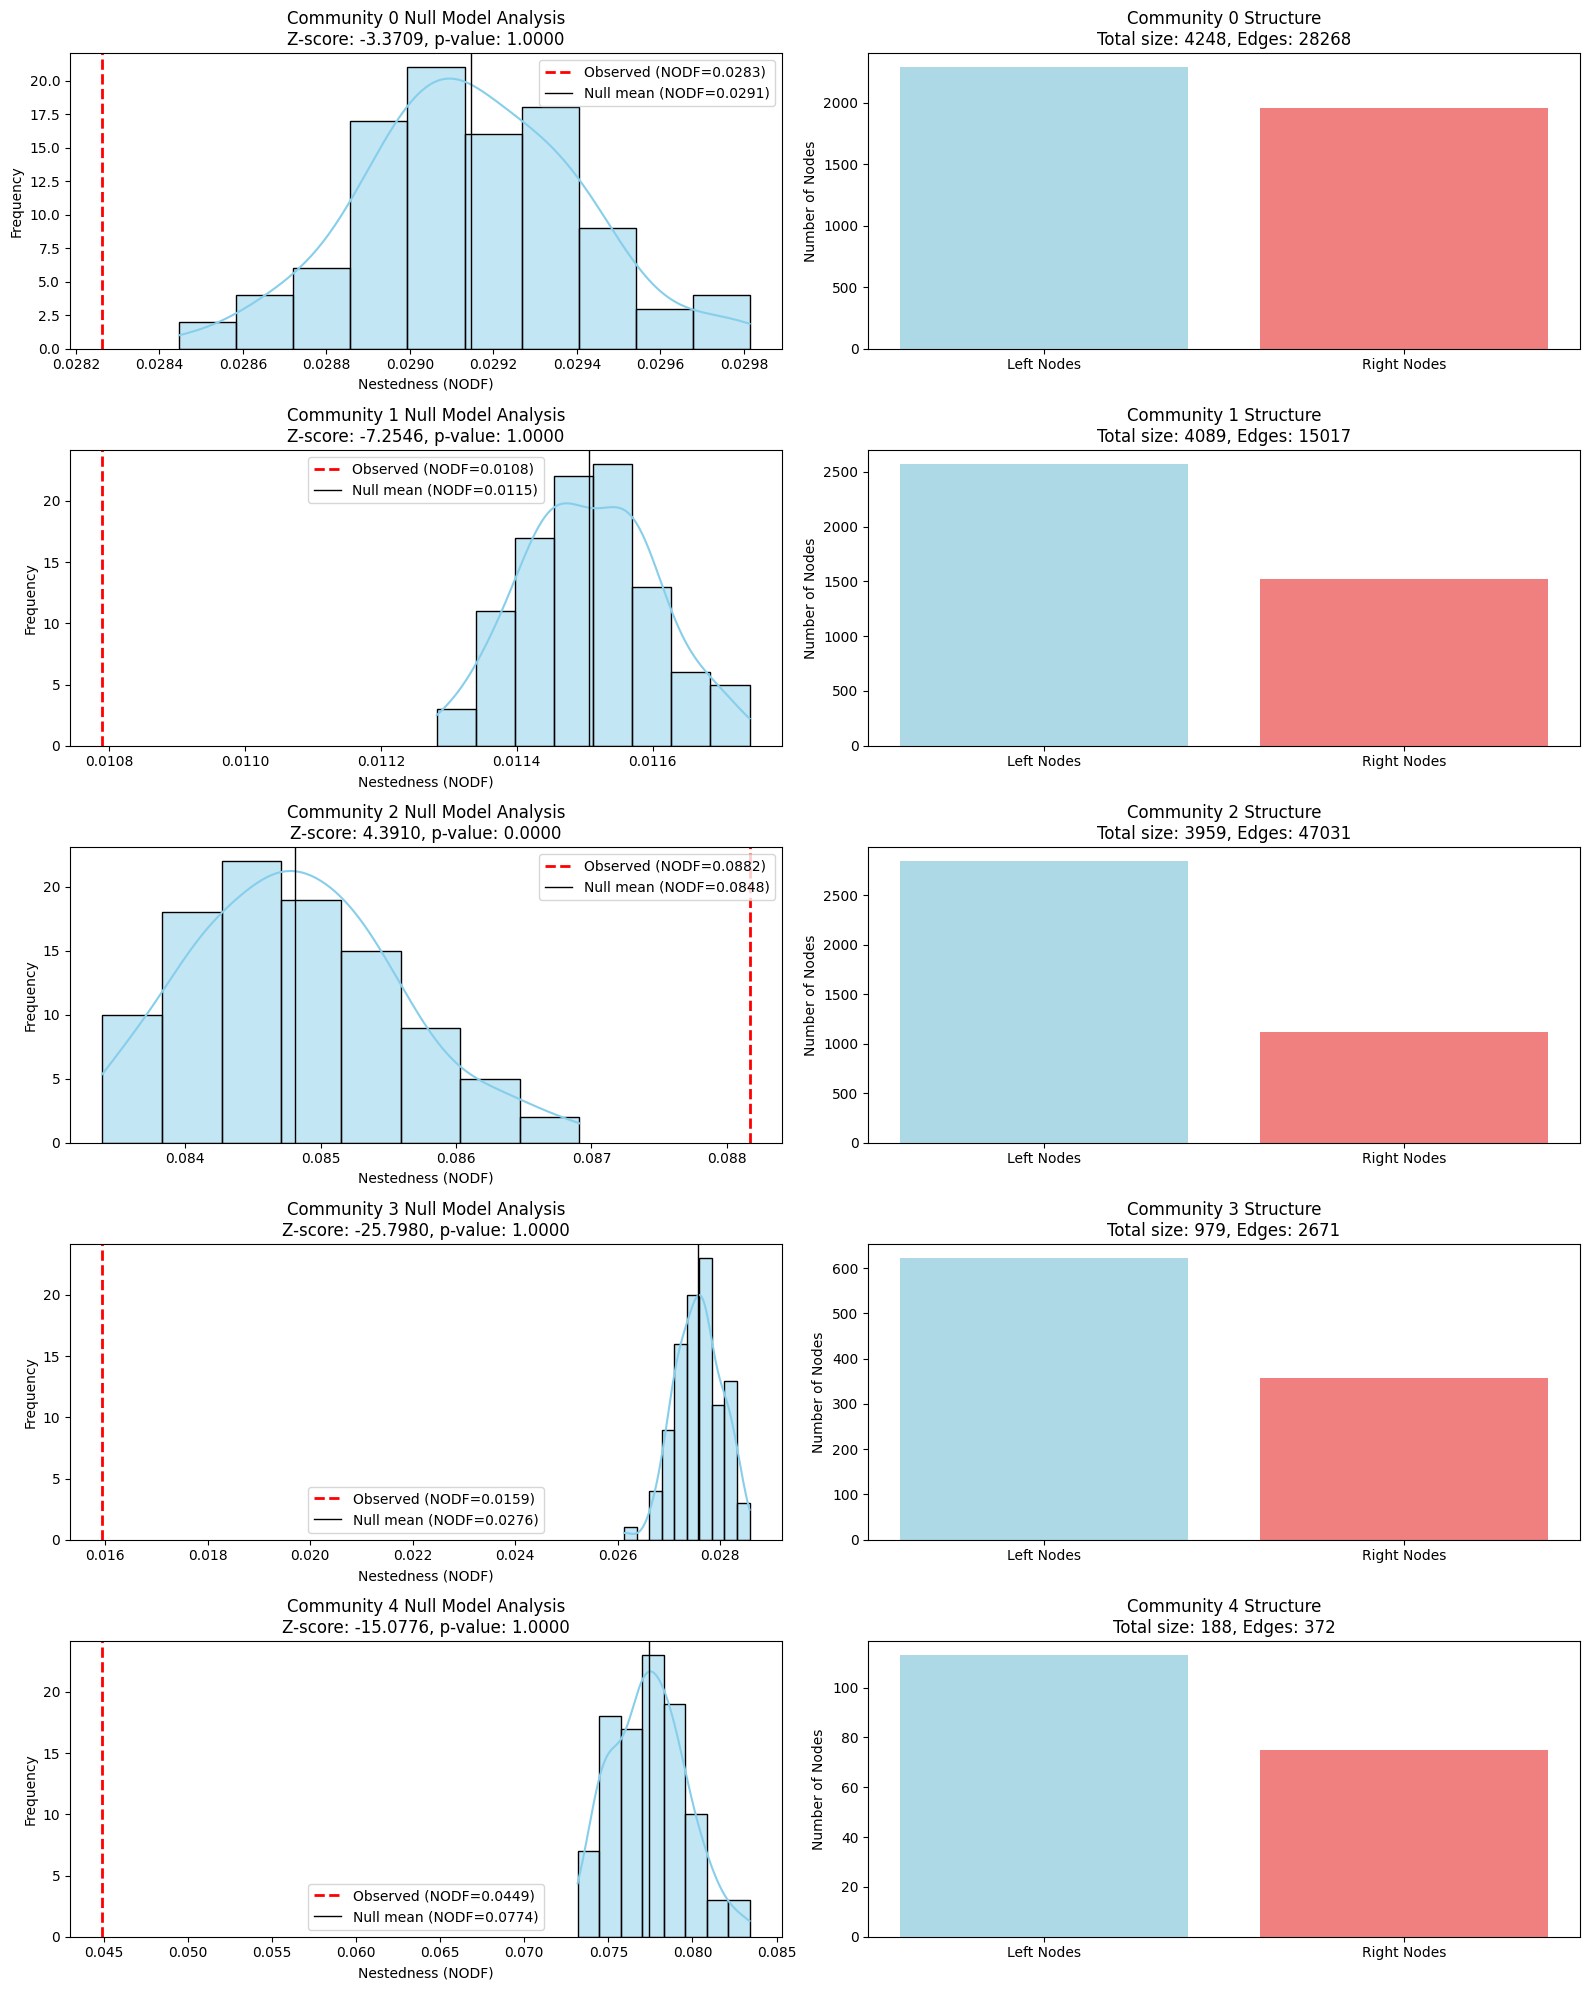
\includegraphics[width=0.8\textwidth]{./assets/null-model-analysis-top-5.png}
\caption{Observed vs null nestedness comparison for the top \numCommAnalysedNestedness{} communities. Each point represents a community, with observed NODF scores plotted against the mean null model NODF scores.}
\label{fig:nestedness_comparison}
\end{figure}

% @todo: analyse Z-score. The distribution of Z-scores across communities indicates that most communities exhibit nestedness levels consistent with random networks, but several communities show substantially higher nestedness than expected by chance.

\newcommand{\interestingCommunity}{2}
\newcommand{\interestingCommunityNODF}{0.088}
\newcommand{\interestingCommunityPValue}{0.00001}

Community \interestingCommunity{} emerges as particularly interesting, showing nestedness score (NODF = \interestingCommunityNODF{}) with strong statistical significance ( p = \interestingCommunityPValue{}). This community demonstrates a clear mutualistic structure where less connected investors tend to co-invest with a subset of the partners of more connected investors.

\subsection{Community Characterization}

Analysis of the geographic and sectoral characteristics of the most nested communities reveals distinct patterns:

@todo: mention only first 3 communities are being compared

\subsubsection{Geographic Distribution}

The highly nested communities show concentration in specific geographic regions, with [DESCRIPTION of geographic patterns].

\begin{figure}[htbp]
\centering
\begin{subfigure}{0.48\textwidth}
    \centering
    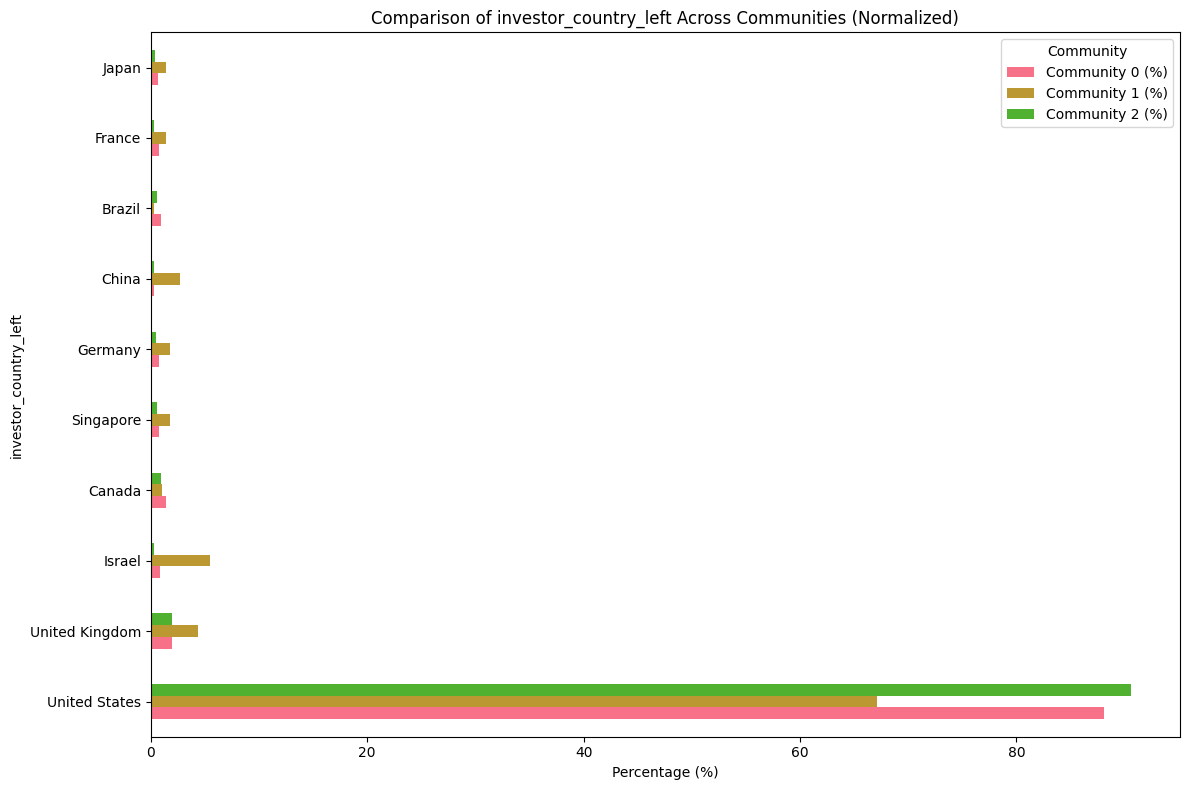
\includegraphics[width=\textwidth]{./assets/investor-left-countries.png}
    \caption{Late-stage investors geographic distribution}
    \label{fig:late_stage_geo}
\end{subfigure}
\hfill
\begin{subfigure}{0.48\textwidth}
    \centering
    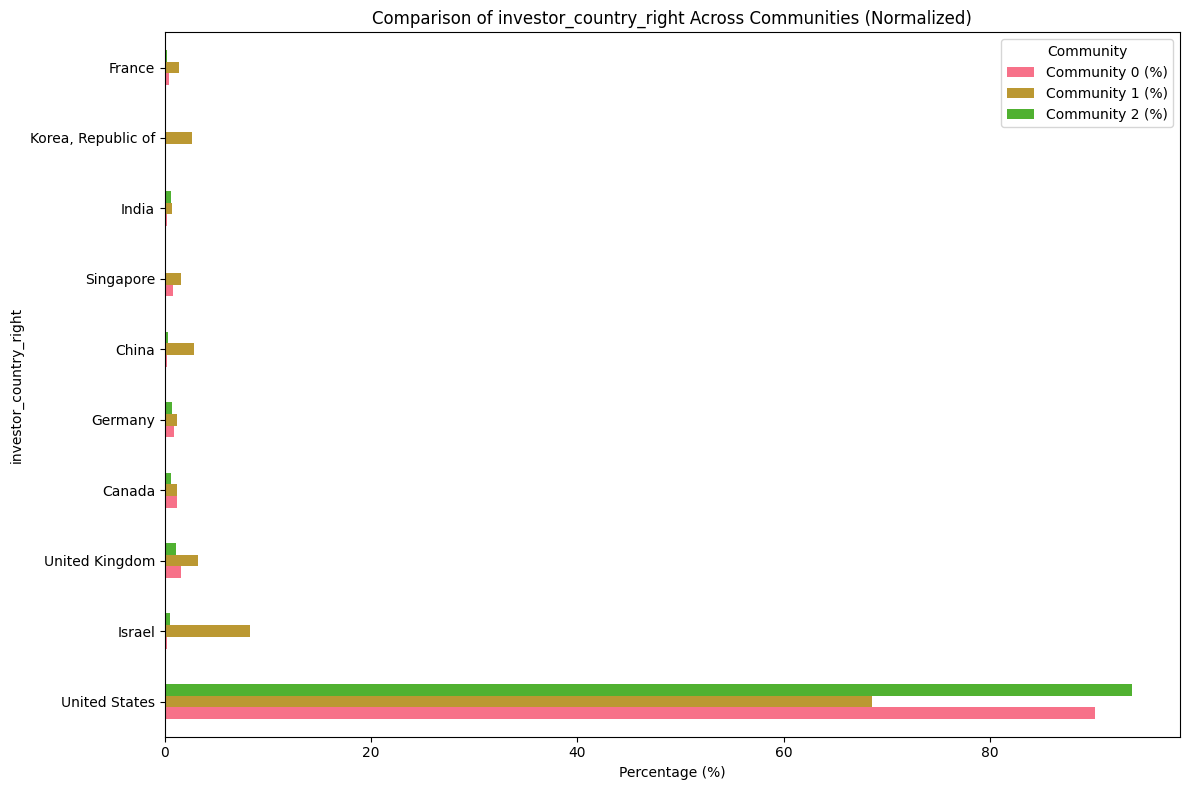
\includegraphics[width=\textwidth]{./assets/investor-right-countries.png}
    \caption{Early-stage investors geographic distribution}
    \label{fig:early_stage_geo}
\end{subfigure}
\caption{Geographic distribution of venture capital investors across the largest communities, showing distinct regional clustering patterns between late-stage (left) and early-stage (right) investor groups.}
\label{fig:geographic_distribution}
\end{figure}

\subsubsection{Investment Stage Preferences}

Communities differ in their focus on specific investment stages. The most nested community shows [DESCRIPTION of stage preferences].

Figure \ref{fig:investment_stage_distribution} illustrates the distribution of investment stages within each community, revealing distinct patterns in how early-stage and late-stage investors are distributed across different funding rounds.

\begin{figure}[htbp]
\centering
\begin{subfigure}{0.48\textwidth}
    \centering
    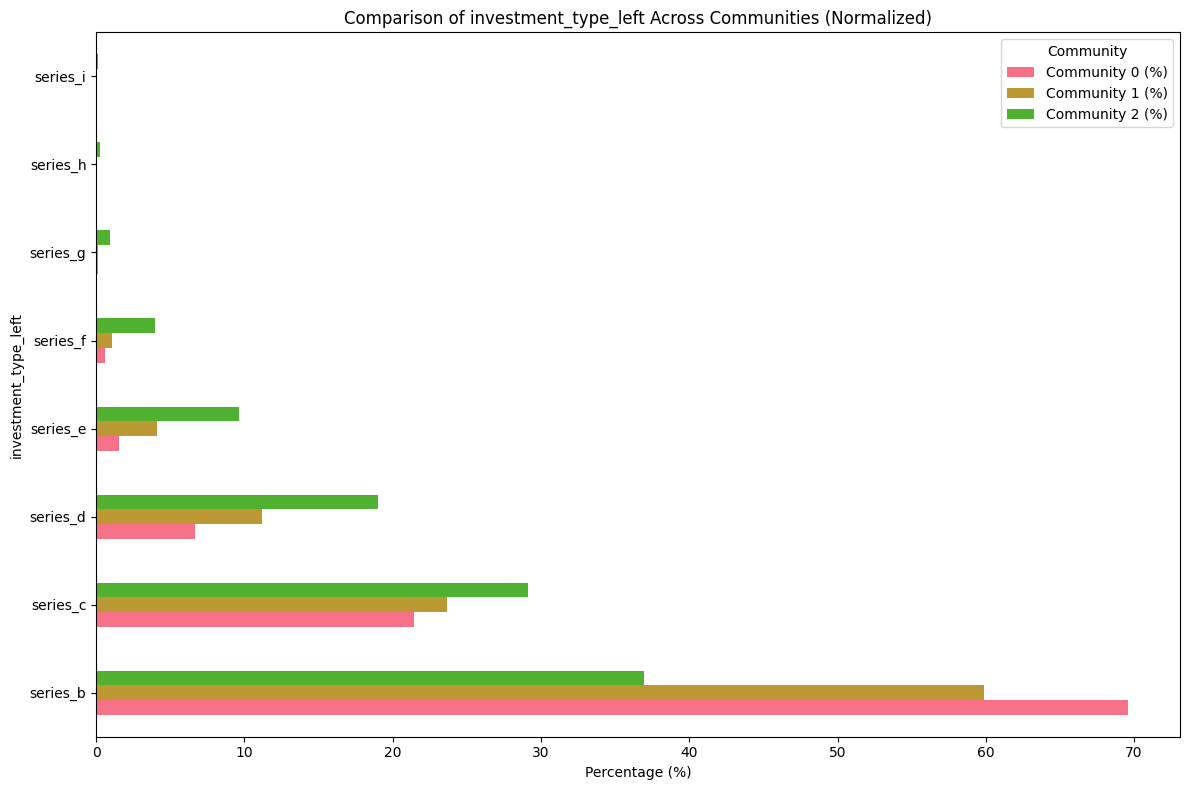
\includegraphics[width=\textwidth]{./assets/late-investment-types-distribution.png}
    \caption{Late-stage investment types distribution}
    \label{fig:late_stage_types}
\end{subfigure}
\hfill
\begin{subfigure}{0.48\textwidth}
    \centering
    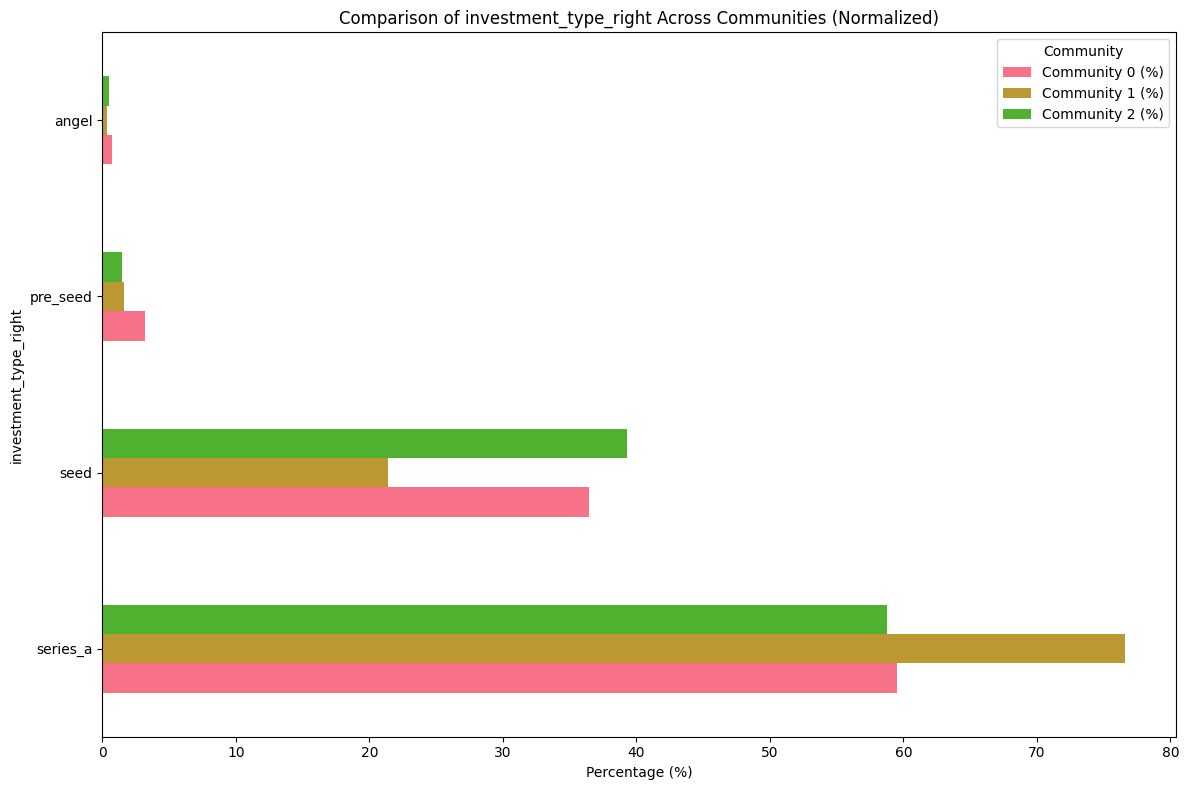
\includegraphics[width=\textwidth]{./assets/early-investment-types-distribution.png}
    \caption{Early-stage investment types distribution}
    \label{fig:early_stage_types}
\end{subfigure}
\caption{Investment stage preferences across the largest communities, showing the distribution of investment types for late-stage (left) and early-stage (right) investor groups.}
\label{fig:investment_stage_distribution}
\end{figure}

\subsubsection{Sectoral Focus}

Sectoral analysis reveals that nested communities often specialize in particular technology sectors or industries.

\begin{figure}[htbp]
\centering
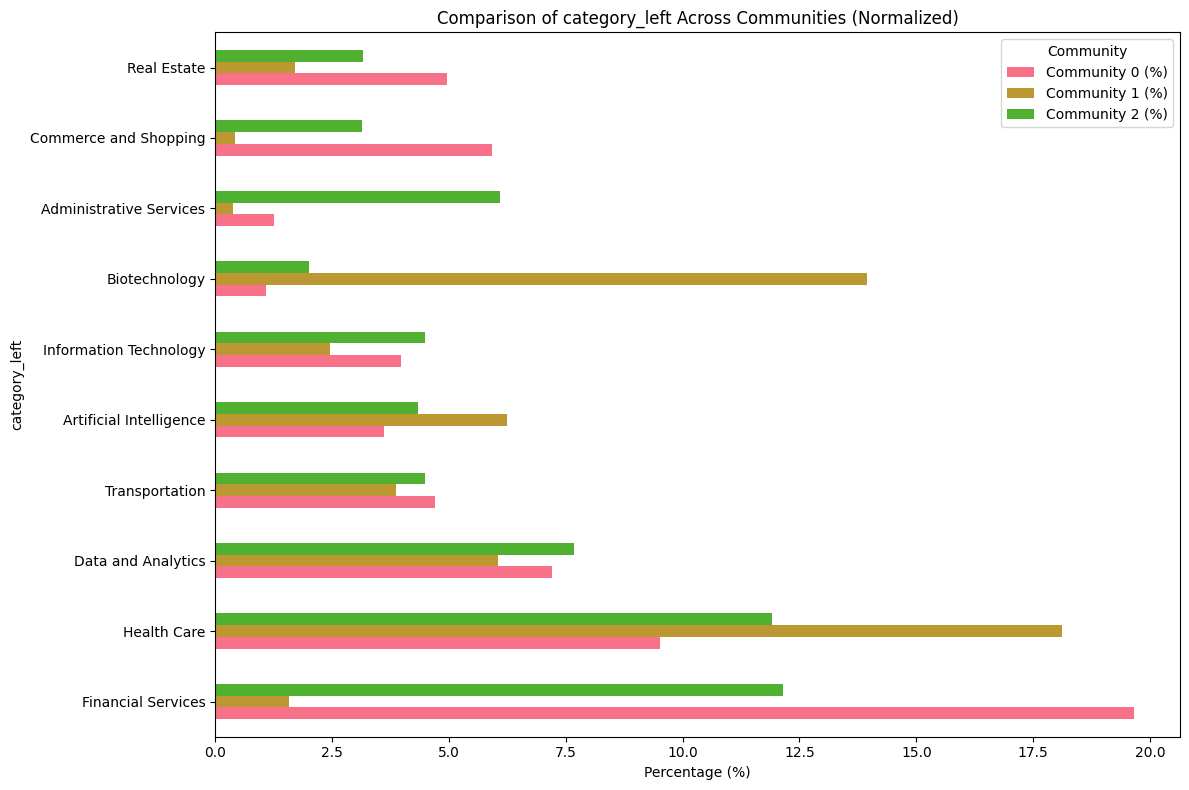
\includegraphics[width=0.8\textwidth]{./assets/sectorial-distribution.png}
\caption{Sectoral distribution across the largest communities, showing industry specialization patterns within different investor groups.}
\label{fig:sectoral_distribution}
\end{figure}

\subsubsection{Funding Characteristics}

The funding patterns within nested communities differ from random networks, with [DESCRIPTION of funding patterns].

\begin{figure}[htbp]
\centering
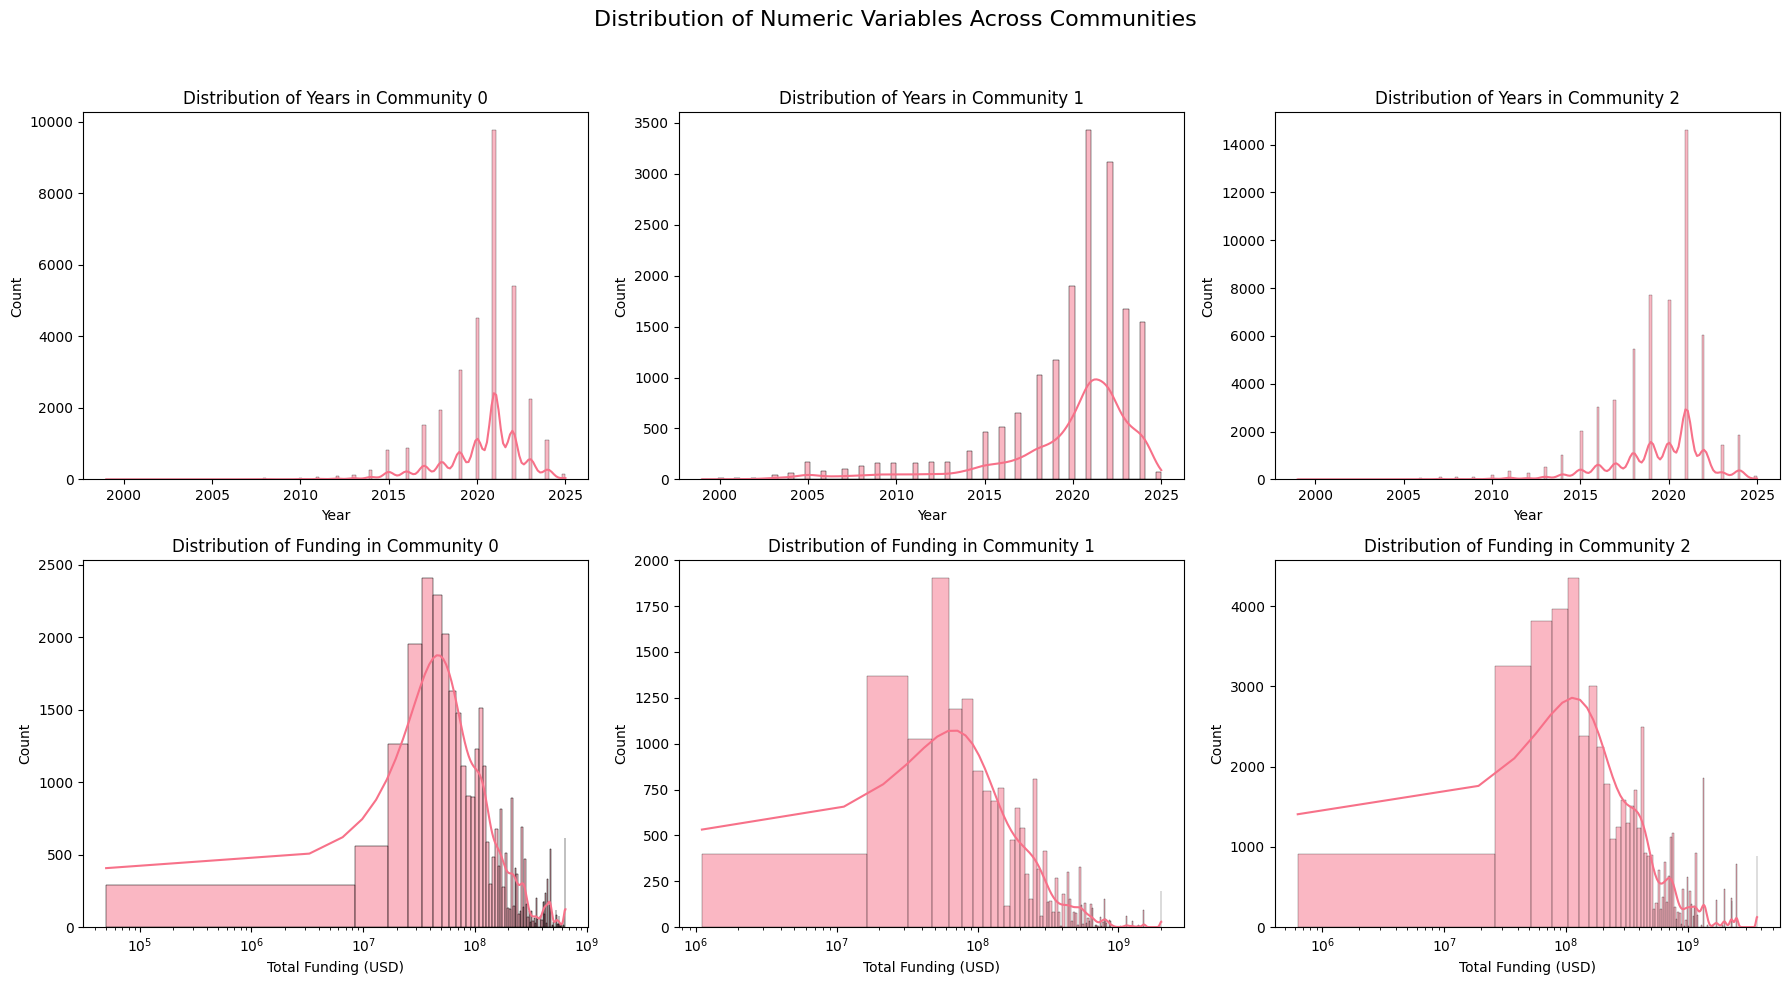
\includegraphics[width=0.8\textwidth]{./assets/funding-characteristics.png}
\caption{Funding characteristics across the largest communities, showing distribution patterns of funding amounts and investment frequency within different investor groups.}
\label{fig:funding_characteristics}
\end{figure}

\subsection{Implications and Future Directions}

The discovery of significantly nested communities within the venture capital network has important implications for understanding investor behavior and startup access to capital. The hierarchical structure observed in these communities suggests the existence of informal investment hierarchies that may influence funding accessibility for entrepreneurs.

@todo: Investigate the economic consequences of nested community structure on startup success rates and funding efficiency.

@todo: Analyze the temporal evolution of community nestedness to understand how these structures emerge and persist over time.

@todo: Examine whether nested communities provide better or worse outcomes for portfolio companies compared to random investment patterns.

The presence of nested structures challenges the assumption of random mixing in venture capital markets and suggests that certain investors may serve as "gatekeepers" who influence access to broader investment networks. This finding aligns with social network theories about structural holes and brokerage positions \cite{Borgatti2011}.

@todo: Apply social network theories of structural holes to understand the role of highly connected investors in nested communities.

@todo: Investigate whether the nested structure reflects information asymmetries or risk-sharing mechanisms among investors.

The identification of these nested communities opens several avenues for future research into the social and economic mechanisms that drive venture capital ecosystem organization. Understanding these patterns may inform policy discussions about startup ecosystem development and investor network formation.

@todo: Develop theoretical models to explain the emergence of nested structures in investment networks.

@todo: Compare nestedness patterns across different geographic markets and time periods to understand generalizability.

This analysis provides the foundation for deeper investigation into how nested investor communities influence entrepreneurial ecosystems and capital allocation efficiency, which will be the focus of subsequent research phases.

\bibliographystyle{plain}
\bibliography{references}

\end{document}